\documentclass[12pt]{article} % The document class with options

\usepackage[margin=1in]{geometry}
\usepackage[utf8]{inputenc} 
\geometry{a4paper}
\usepackage{newtxtext,newtxmath}
\usepackage[T1]{fontenc}
\usepackage{amsmath}
\usepackage{amsfonts}
\usepackage{microtype}
\usepackage{graphicx}
\usepackage{listings} % For formatting and highlighting code
\usepackage{color}    % For colors in code highlighting

% Define colors for syntax highlighting
\usepackage{color}
\definecolor{dkgreen}{rgb}{0,0.6,0}
\definecolor{gray}{rgb}{0.5,0.5,0.5}
\definecolor{mauve}{rgb}{0.58,0,0.82}

% Code listing style named "mystyle"
\lstset{frame=tb,
  language=Python,
  aboveskip=3mm,
  belowskip=3mm,
  showstringspaces=false,
  columns=flexible,
  basicstyle={\small\ttfamily},
  numbers=none,
  numberstyle=\tiny\color{gray},
  keywordstyle=\color{blue},
  commentstyle=\color{dkgreen},
  stringstyle=\color{mauve},
  breaklines=true,
  breakatwhitespace=true,
  tabsize=3
}
% chktex-file 3
% chktex-file 8
% chktex-file 10
% chktex-file 17
% chktex-file 18
% chktex-file 36
% chktex-file 44

\begin{document}
\setlength{\parskip}{1em} 
\setlength{\parindent}{0pt}
\newcommand{\vect}[1]{\mathbf{#1}}

\begin{titlepage}  % This starts a title page environment
    \centering    % Center everything on the page

    %--- Add space at the top of the page ---
    \vspace*{2cm}
    
    %--- Title ---
    \normalsize \textbf{CHBE 552 Project Report} \\
    \vspace{0.5cm}  % Space between lines
    \normalsize\textbf{Comparison of Gauss-Newton Method with Marquardt Modification with \\
     Nelder-Mead Algorithm for Parameter Estimation in Algebraic Models} \\
    \vspace{2cm}  % Space between the title and the author name
    
    %--- Author ---
    \normalsize by\\
    \vspace{1cm}
    \normalsize Jincong Li \\ 
    \vspace{1cm}
    \normalsize M.Eng, The University of British Columbia, 2024
    \vspace{11cm}  % Space between the author and the date
    
    %--- Date ---
    \normalsize \today

    \vfill  % Push the following content to the bottom of the page
    %--- Bottom part of the page ---
    © Jincong Li, 2024
\end{titlepage}
\tableofcontents
\newpage
\section{Abstract}
This project report presents a comprehensive comparison of two parameter estimation methods, the Gauss-Newton method with Marquardt modification and the Nelder-Mead algorithm, as applied to two specific algebraic models in chemical engineering. These models relate to the adsorption of 1,2-Dichloropropane on Activated Carbon and the kinetics of MnO2-catalyzed Acetic Acid oxidation in supercritical water. The objective is to evaluate and compare the effectiveness of these optimization methods in accurately estimating the parameters of these models based on their performance, including the reliability of the estimated parameters as expressed through confidence intervals. The methods were implemented in Python, and parameter estimation was performed on experimental data from referenced studies. The study highlights the challenges and effectiveness of each method under the constraints of the complex algebraic models used in chemical engineering, providing insights into their practical applications and limitations.
\section{Introduction}
Parameter estimation plays a crucial role in modeling and understanding various processes across
engineering and science disciplines. Accurate estimation of model parameters allows for the
prediction and optimization of system behavior. This project aims to compare the effectiveness
of two widely used optimization methods, Gauss-Newton method with Marquardt modification and Nelder-Mead Algorithm,
in estimating parameters of algebraic models. The comparison will be based on solving two
distinct chemical engineering problems: 1) Adsorption of 1,2-Dichloropropane on Activated
Carbon[1], and 2) Kinetics of MnO2-Catalyzed Acetic Acid Oxidation in Supercritical Water[2].
Note that the chemical nature of these two problems is not the main focus of this project, 
so the meaning of each variable is omitted in the following sections. The problems are treated
as pure algebraic models.
\subsection{Adsorption of 1,2-Dichloropropane on Activated Carbon}
The algebraic model is given by
\begin{equation}
    q = \frac{q_{\text{sat}} \cdot k \cdot p}{(1 + (k \cdot p)^t)^{\frac{1}{t}}}
\end{equation}
where \( p \) is the input variable, \( q \) is the output variable, and \( q_{\text{sat}}, k, t \) are parameters of the model.
\subsection{Kinetics of MnO2-Catalyzed Acetic Acid Oxidation in Supercritical Water}
The algebraic model for the second problem is given by
\begin{equation}
    W_{F_A0} = \frac{(1 + k_3 \cdot [O_2])^2 \cdot (k_2 \cdot [HOAC] \cdot X - \ln(1-X))}{k_1 \cdot [HOAC] \cdot [O_2]}
\end{equation}
where \( W_{F_A0} \) is the input variable, \( X \) is the output variable, and \( k1, k2, k3 \) are parameters of the model.

As mentioned, this work will investigate into comparing two different optimization method in parameter estimation for algebraic models over two well-studied cases. One method is chosen from the gradient-based methods, that is the Gauss-Newton method with Marquardt modification. The other method is the Nelder-Mead algorithm which
is a kind of Simplex methods from the direct search field. They will be briefly reviewed here as well as the methods for computing the confidence intervals. 
\subsection{The Gauss-Newton Method with Marquardt Modification}

\subsubsection{Gauss-Newton Method}

The Gauss-Newton method is an algorithm used for solving non-linear least squares problems, which are often encountered in parameter estimation for algebraic models. This method iteratively refines parameter estimates to minimize the sum of squared differences between observed and model-predicted values.

\subsubsection{Formulation}
Given a set of observations $y_i$ and a non-linear model $f(x_i, \beta)$, where $x_i$ are the independent variables and $\beta$ represents the parameters to be estimated, the objective is to minimize the sum of squared residuals $S(\beta)$ defined as:
\[
S(\beta) = \sum_{i=1}^n \left(y_i - f(x_i, \beta)\right)^2
\]
The parameter updates in each iteration are calculated using:
\[
\beta_{\text{new}} = \beta_{\text{old}} + (J^T J)^{-1} J^T r
\]
Here, $J$ is the Jacobian matrix of partial derivatives of the model functions with respect to the parameters $\beta$, and $r$ is the vector of residuals between the observed and predicted values.

\subsubsection{Marquardt's Modification (Levenberg-Marquardt Algorithm)}

The Levenberg-Marquardt algorithm modifies the Gauss-Newton method by introducing a damping factor $\lambda$ to improve the convergence properties, especially in situations where the Jacobian matrix $J^T J$ is not invertible or near singular. The updated formula for parameter adjustment becomes:
\[
\beta_{\text{new}} = \beta_{\text{old}} + (J^T J + \lambda I)^{-1} J^T r
\]
Here, $I$ is the identity matrix. The value of $\lambda$ adjusts dynamically during iterations: when $\lambda$ is high, the algorithm behaves more like gradient descent, taking smaller steps; when $\lambda$ is low, it behaves more like the Gauss-Newton method, taking larger, more aggressive steps.

\subsubsection{Application}
The essence of Marquardt's modification is to combine the strengths of both the Gauss-Newton method and gradient descent, allowing for a more versatile and robust approach to parameter estimation in non-linear models. The algorithm iteratively adjusts $\lambda$ and the parameters $\beta$ until convergence is reached, typically when the change in the sum of squared residuals is below a certain threshold.

%\textbf{Summary:} The Levenberg-Marquardt algorithm is a powerful tool for parameter estimation in non-linear models, offering a compromise between the speed of Gauss-Newton and the stability of gradient descent. It is widely used in various scientific and engineering applications where accurate parameter estimation is crucial.
\subsection{Computing Confidence Intervals for Estimated Parameters}

The confidence interval information of the estimated parameters is also required in this work, since it could indicate the relibility of the parameter values estimated by optimization method, such as the Gauss-Newton method with Marquardt modification. The confidence intervals for the estimated parameters are computed based on the statistical properties of the least squares estimators, using their standard errors and the assumption that they follow a t-distribution, especially in the context of small sample sizes.

\subsubsection{Steps to Compute the Confidence Intervals}

\begin{enumerate}
    \item \textbf{Covariance Matrix Calculation:}
    \begin{itemize}
        \item After obtaining the parameter estimates through an optimization process such as the Gauss-Newton method (modified by Marquardt), calculate the covariance matrix of the parameter estimates.
        \item This matrix is derived from the inverse of the Hessian matrix, which in the context of the Gauss-Newton method, is approximated by $J^T J$, where $J$ is the Jacobian matrix of the partial derivatives of the residuals with respect to the parameters.
        \item If $J^T J$ is singular or near-singular, indicating potential issues with model identifiability or data collinearity, use the pseudo-inverse for stability.
    \end{itemize}
    \item \textbf{Standard Errors of the Parameter Estimates:}
    \begin{itemize}
        \item The diagonal elements of the covariance matrix provide the variances of the parameter estimates.
        \item The standard errors of the estimates are obtained by taking the square root of these diagonal elements.
    \end{itemize}
    \item \textbf{Confidence Interval Calculation:}
    \begin{itemize}
        \item With the standard errors, compute the confidence intervals for the parameters.
        \item For a specified confidence level (e.g., 95\%), determine the critical value from the t-distribution, considering the degrees of freedom, which typically depend on the number of data points and the number of parameters.
        \item The confidence interval for each parameter is calculated as:
        \[
        \text{Parameter Estimate} \pm (t\text{-critical value} \times \text{Standard Error})
        \]
    \end{itemize}
\end{enumerate}
\subsection{Nelder-Mead Algorithm}
The Nelder-Mead algorithm, also known as the Downhill Simplex Method or Amoeba Method, is an optimization method used to find the minimum or maximum of an objective function in a multidimensional space. It is particularly suitable for problems where the objective function does not have a derivative or is not smooth.
\begin{itemize}
    \item \textbf{Initialization:} Start with a simplex, which in two dimensions is a triangle and in three dimensions is a tetrahedron. This simplex is formed by $n+1$ vertices for an $n$-dimensional problem, where each vertex represents a potential solution.
    \item \textbf{Evaluation:} Calculate the objective function at each vertex.
    \item \textbf{Transformation:} Perform one of four actions based on the values of the objective function at the vertices:
    \begin{enumerate}
        \item \textbf{Reflection:} Creates a new point by reflecting the worst point of the simplex across the opposite face of the simplex.
        \item \textbf{Expansion:} If the reflection results in a better point, the algorithm tries to take a larger step in the same direction to see if the improvement continues.
        \item \textbf{Contraction:} If reflection does not improve the solution, the algorithm takes a smaller step from the worst point towards the simplex.
        \item \textbf{Shrinkage:} If contraction still does not yield a better point, the algorithm reduces the size of the simplex towards the best current point.
    \end{enumerate}
    \item \textbf{Iteration:} Repeat the evaluation and transformation steps until a stopping criterion is met, such as a minimum change in the objective function value or a maximum number of iterations.
\end{itemize}

\textbf{Note:} The Nelder-Mead method does not require derivatives of the objective function, making it useful for optimization problems where derivatives are difficult or impossible to calculate. However, it is not guaranteed to find the global minimum, especially in problems with multiple local minima.

\subsection{Bootstrap Method for Computing Confidence Intervals}

However, in the Simplex family method, the derivatives are not available, which means the covariance matrix method for computing the confidence interval is not applicable. Thus, we need a new method in this case to capture the confidence interval information. The bootstrap method is a powerful statistical tool used to estimate the distribution of a statistic by resampling with replacement from the original data. It is particularly useful in situations where the theoretical distribution of the statistic is unknown or complex.

\subsubsection{Steps in Bootstrap Method}

\begin{enumerate}
    \item \textbf{Data Resampling:}
    \begin{itemize}
        \item Generate a large number of bootstrap samples from the original dataset by resampling with replacement. Each bootstrap sample is the same size as the original dataset.
    \end{itemize}

    \item \textbf{Statistic Calculation:}
    \begin{itemize}
        \item Calculate the statistic of interest (e.g., mean, median) for each bootstrap sample. This process creates a distribution of the statistic known as bootstrap replicates.
    \end{itemize}

    \item \textbf{Confidence Interval Estimation:}
    \begin{itemize}
        \item \textbf{Percentile Method:} For a 95\% confidence interval, use the 2.5th and 97.5th percentiles of the bootstrap statistics.
        \item \textbf{Bias-Corrected and Accelerated (BCa) Method:} This more complex method adjusts for both bias and skewness in the bootstrap distribution, providing more accurate confidence intervals.
    \end{itemize}

    \item \textbf{Interpretation:}
    \begin{itemize}
        \item The resulting confidence interval estimates where the true parameter lies with a specified level of confidence.
    \end{itemize}
\end{enumerate}

\subsubsection{Advantages of the Bootstrap Method}
\begin{itemize}
    \item Flexible and applicable to various statistics.
    \item Simple to implement with modern computing power.
    \item Nonparametric and does not assume a specific parametric distribution.
\end{itemize}

\subsubsection{Limitations}
\begin{itemize}
    \item Requires a large sample size to be effective.
    \item Computationally demanding due to the need to generate thousands of bootstrap samples.
    \item May not perform well with very small sample sizes or highly skewed data.
\end{itemize}
\section{Methodology}
The two problems and two optimization methods mentioned in the introduction method will be implemented in Python. Key algorithm procedures are described as followings: note that in each step, the
first problem is used as example, the procedure for the second problem will be analogical. 
\begin{enumerate}
    \item \textbf{Model Function:} The algebraic model of the problem will be converted to the model function that could be called by other functions. For instance:
    \begin{lstlisting}
        def model(p, q_sat, k, t):
            # Ensure all operations are element-wise
            p = np.array(p, dtype=float)
            term = (1 + (k * p) ** t)
            return q_sat * k * p / term ** (1 / t)
        \end{lstlisting}

    \item \textbf{Residual Function:} For the Levenberg-Marquardt algorithm, this function calculates the residual between the estimated output and the experiment output.
    \begin{lstlisting}
    def residual(params, p, q_obs):
    q_sat, k, t = params
    return q_obs - model(p, q_sat, k, t)
    \end{lstlisting}
    This function calculates the difference between observed values \( q_{\text{obs}} \) and the model predictions.

    \item \textbf{Jacobian Matrix Calculation:}
    The Jacobian matrix of the model with respect to the parameters \( q_{\text{sat}}, k, t \) is calculated for optimization. Detailed implementation is omitted here since the partial derivatives are too long to fit in.

    \item \textbf{Levenberg-Marquardt Algorithm/Nelder-Mead Algorithm:} Levenberg-Marquardt Algorithm is shown here as an example, the implementation for Nelder-Mead Algorithm will be analogical.
    
    %The algorithm iteratively adjusts the model parameters to minimize the sum of squared residuals. It involves:
    \begin{lstlisting}
        def levenberg_marquardt(p, q, params_guess, max_iter=100, lambda_inc=10, lambda_dec=10, lambda_init=0.01):
        params = np.array(params_guess, dtype=float)
        n = len(q)
        iteration_details = []
    
        # Initial calculation
        r = residual(params, p, q)
        J = jacobian(p, params)
        
        A = J.T @ J
        g = J.T @ r
        lambda_ = lambda_init * np.max(np.diag(A))
        objective = np.sum(r**2)
    
        for i in range(max_iter):
            # Solve for parameter update
            try:
                delta = np.linalg.solve(A + lambda_ * np.eye(len(params)), g)
            except np.linalg.LinAlgError:
                print(f"Iteration {i}: Singular matrix encountered. Adjusting lambda.")
                lambda_ *= lambda_inc
                continue
                # Check if improvement
                new_params = params + delta
                new_r = residual(new_params, p, q)
                new_objective = np.sum(new_r**2)
            \end{lstlisting}

    \item \textbf{Parameter Adjustment and Convergence Checking:}
    Parameters are updated based on improvement in the objective function, iterating until convergence criteria are met.
    \begin{lstlisting}
        
        if new_objective < objective:
            # Update is successful, decrease lambda (move towards Gauss-Newton method)
            lambda_ /= lambda_dec
            params = new_params
            objective = new_objective
            r = new_r
            J = jacobian(p, params)
            A = J.T @ J
            g = J.T @ r
            #print(f"Iteration {i}: Success - Parameters updated to: {params} with objective: {objective}")
        else:
            # Update is not successful, increase lambda (move towards gradient descent)
            lambda_ *= lambda_inc
            #print(f"Iteration {i}: No improvement - Lambda adjusted to: {lambda_}")
    \end{lstlisting}
    \item \textbf{Error Estimation (Confidence Interval Computation):}
    Post-fitting, the covariance matrix of the parameters is calculated using the Jacobian matrix from the final iteration to estimate their standard errors for Levenberg-Marquardt Algorithm.
    And the bootstrap method applied for Nelder-Mead Algorithm is shown here as an example:
    \begin{lstlisting}
    def bootstrap_CI(data, model_func, optimization_func, initial_guesses, n_iterations=1000, ci=95):

    np.random.seed(42)  # For reproducibility
    p_data, q_data = data
    estimates = []

    for _ in range(n_iterations):
        # Bootstrap sample
        bs_indices = np.random.choice(range(len(p_data)), size=len(p_data), replace=True)
        bs_p_data = p_data[bs_indices]
        bs_q_data = q_data[bs_indices]
        
        # Update objective function for bootstrap sample
        def bs_objective_function(params):
            predicted_q = model_func(bs_p_data, *params)
            return np.sum((bs_q_data - predicted_q) ** 2)
        
        # Estimate parameters for bootstrap sample
        bs_estimates = optimization_func(bs_objective_function, initial_guesses)
        estimates.append(bs_estimates)
    
    # Calculate confidence intervals
    estimates = np.array(estimates)
    lower_bounds = np.percentile(estimates, (100 - ci) / 2, axis=0)
    upper_bounds = np.percentile(estimates, 100 - (100 - ci) / 2, axis=0)
    
    return list(zip(lower_bounds, upper_bounds))
    \end{lstlisting}
    \item \textbf{Handling Multiple Data Sets \& Execution \& Post-Processing:}
    The implementation is set up to handle multiple data sets for different scenarios, each characterized by different initial parameters and data points. Then the algorithm functions will be called
    by specifying corresponding initial guess and experiment data, and the result of estimated values of parameters will be returned as well as the confidence interval information. Finally, those results will be 
    printed to the console and the comparison between experiment data and estimated data will be plotted as well.
    \item \textbf{Special Treatment for Problem 2:}
    In this problem, as we can see in the definition of the model, the output variable X is included in the RHS of the model (even in a $Log$), which
    means that it could not be solved explicitly, and this fact requires the code to solve for X numerically and the numerical solver package
    "scipy.optimize.brentq" is applied. 
    \begin{lstlisting}
        def inverse_model_function_bounded(W_F_A0, k1, k2, k3):
        """
        Numerically solve for X given W_F_A0 using a bounded solver.
        """
        # Define the equation to solve
        def equation(X):
            return ((1 + k3 * O2)**2) * (k2 * HOAC * X - np.log(1 - X)) / (k1 * HOAC * O2) - W_F_A0
        
        # Use brentq for solving within bounds, providing more stability near edges
        try:
            X_solution = brentq(equation, 0.0001, 0.9999)  # Avoiding exact 0 or 1 to prevent log issues
            return X_solution
        except ValueError as e:
            print(f"No solution found for W_F_A0={W_F_A0} within the bounds: {e}")
            return np.nan  # Return NaN if no solution is found
    
    \end{lstlisting}
\end{enumerate}

\newpage
\section{Result}
The experiment data that the code will intake as input as provided in the reference paper, and they are presented in the Appendix.
\subsection{ Adsorption of 1,2-Dichloropropane on Activated Carbon}
\begin{table}[ht]
    \caption{Results of Parameter Estimation for Problem 1}
    \centering
    \begin{tabular}{|c|c|c|c|c|}
    \hline
Method & Cases($T$) &$q_{sat}$  & $k$ & $t$\\ \hline
GNM & 303 &4.31 ± 0.19& 17.73 ± 5.73& 0.46 ± 0.05\\
& 338 &5.2 ± 0.56& 7.99 ± 2.6& 0.37 ± 0.05\\
& 373 &4.56 ± 1.09& 1.72 ± 0.41& 0.38 ± 0.07\\
& 423 &6.77 ± 6.75& 0.8 ± 0.23& 0.28 ± 0.13\\
& 473 &4.41 ± 12.2& 0.27 ± 0.17& 0.3 ± 0.32\\ \hline
NMA & 303 &4.31[4.25  4.47]& 17.81[16.21 20.28]& 0.45[0.43  0.47]\\
& 338 &5.58[5.21 5.29]& 9.99[7.82 9.2 ]& 0.34[0.33 0.36]\\
& 373 &5.68[5.65 5.68]& 2.1[1.98 2.21]& 0.33[0.32 0.33]\\
& 423 &5.77[5.38 5.85]& 0.74[0.73 0.78]& 0.31[0.3  0.31]\\
& 473 &2.92[2.82 2.99]& 0.3[0.26 0.32]& 0.35[0.34 0.37]\\\hline
\end{tabular}
\label{tab:iteration_details}
\end{table}
Note that "GNM" refers to Gauss-Newton Method with Marquardt Modification and "NMA" refers to Nelder-Mead Algorithm.
And the bracket following the values in NMA is the 95\% confidence interval since the uncertainties are not symmetric.

As presented in table 1, the estimated parameter values from two methods as listed, notice for both methods, same initial guess of parameters are used to ensure the comparability. Comparing with the values reported by the reference (shown in figure 1 below), GNM estimate the parameters perfectly for the first three cases (303T, 338T, and 373T), the estimated values are
exactly the same as reported in the reference with little larger 95\% confidence intervals which is acceptable since they are generally reasonable. For the last two cases, GNM returns the parameters slightly different from 
the reference values with much larger 95\% confidence intervals which are not reasonable. Especially for $q_{sat}$, the uncertainties are even larger than the value of the parameters itself. Contrastively, NMA predicts the parameters for
the last two cases better even though some error still exist but the smaller 95\% confidence intervals indicates its reliability. NMA also successfully estimates the parameter in first three case with some error appears. Comparison between experiment data and estimated data are plotted in
figure 2 and 3. In conclusion, GNM and NMA both estimate the parameter values rationally, but their performance might depend on the input data structure/distribution. One method could be better over the other one in some scenarios just as what we observed in the problem 1. 

Regarding the complexity of
implementation, they are competitive. GNM requires careful treatment of the derivatives/Jacobian Matrix especially when the algebraic model is complex, whereas NMA requires the implementation of additional method for extracting the confidence interval information. Computation time demanded by both
method are less than one minute to estimate the parameters, however, since NMA requires the Bootstrap method to compute the confidence interval which involves resampling the data up to the chosen iteration, it might require much more time if the iteration limit is large.
\begin{figure}[ht]
    \centering
    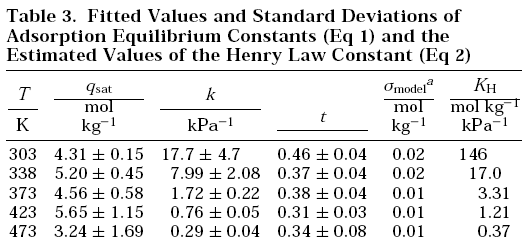
\includegraphics[width=0.8\textwidth]{Q1_ref.png}
    \caption{Parameter Values Reported in Reference for Problem 1[1]}
\end{figure}


\begin{figure}[ht]
    \centering
    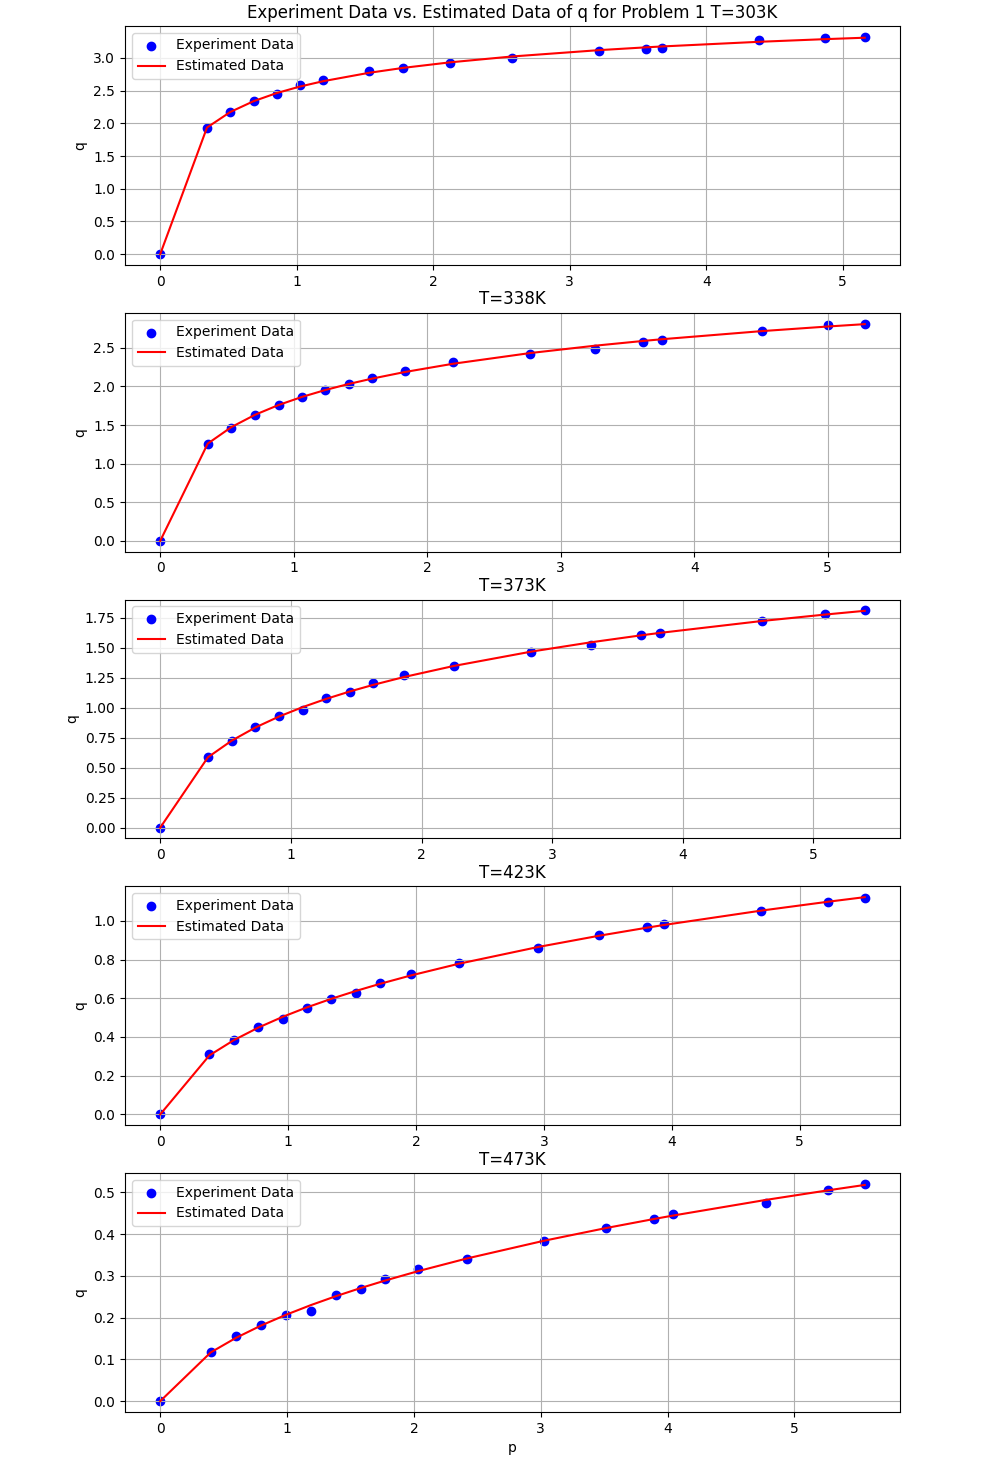
\includegraphics[width=1\textwidth]{Q1_GMN_comp.png}
    \caption{Experiment Data vs. Estimated Data of q for Problem 1 by GNM}
\end{figure}
\clearpage

\begin{figure}[ht]
    \centering
    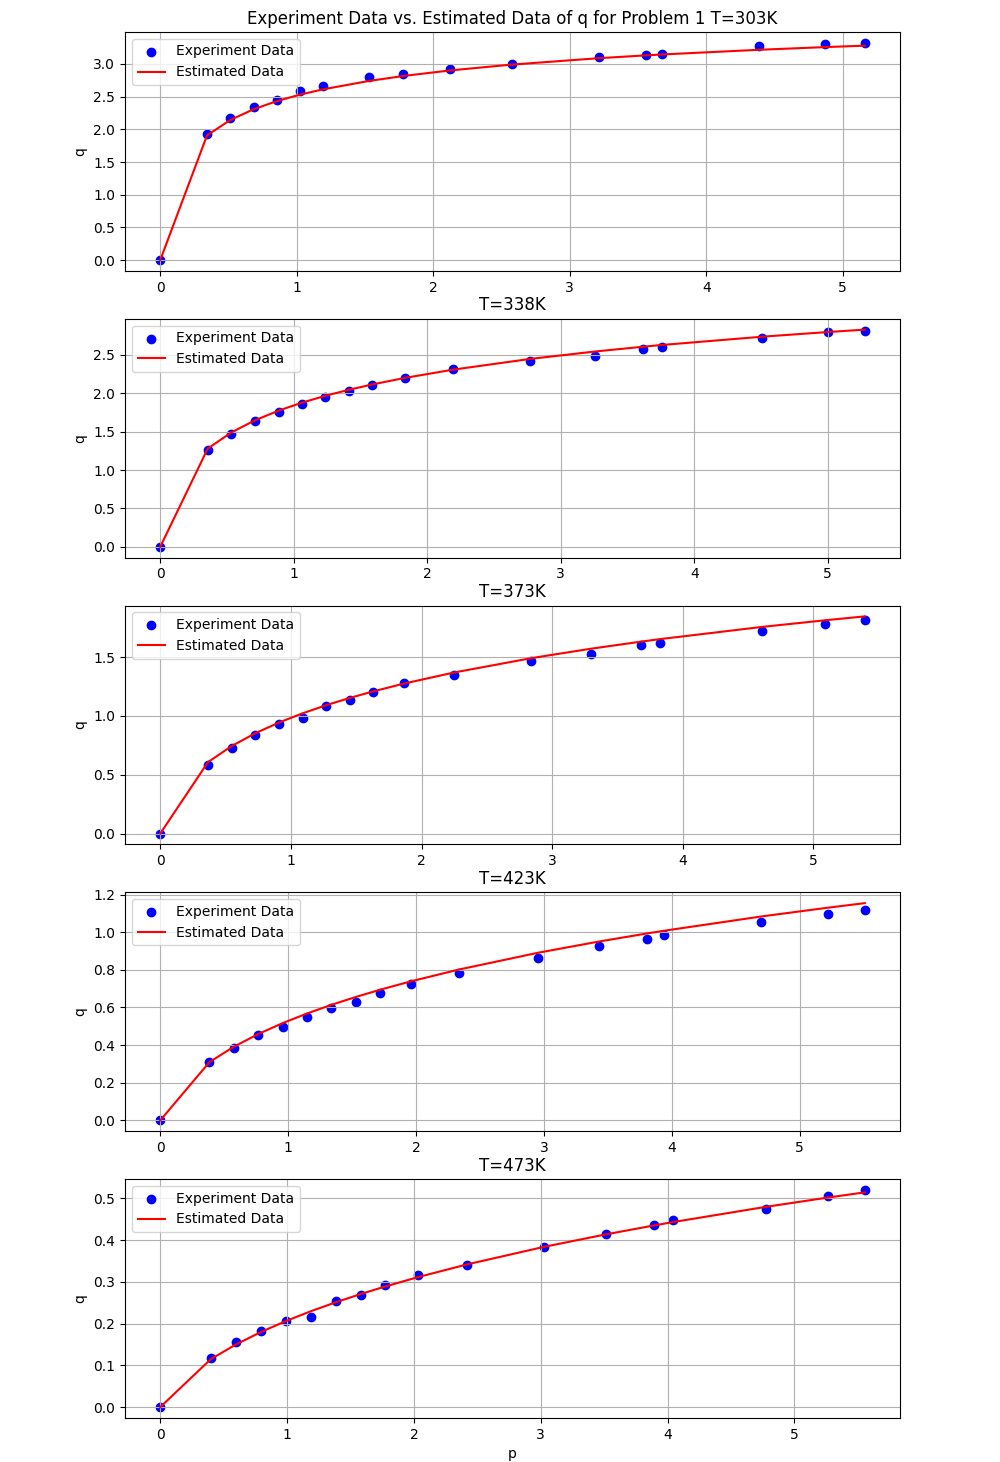
\includegraphics[width=1\textwidth]{Q1_NMA_comp.png}
    \caption{Experiment Data vs. Estimated Data of q for Problem 1 by NMA}
\end{figure}


\clearpage
\subsection{Kinetics of MnO2-Catalyzed Acetic Acid Oxidation in Supercritical Water}
As shown in figure 8 in Appendix, the experiment data varies a lot in terms of reaction temperature, pressure, and concentrations of species. Since the model itself is complex enough and for the performance of the code,
only experiment data for $\frac{W}{F_{A0}} $and $X$ (HOAC convert percentage) in the cases where[$HOAC$] = 3.2 and [$O_2$] = 24 are used. Table 2 below presents the estimated values of parameters, and one can observe that
they do not generally agree across methods. Figure 4 shows the reference values for those parameters which vary in 4 degree of magnitude, which I could not reasonably interpret. Thus, the validation is conducted by comparing 
the experiment data with the estimated data (as shown in figure 5 and 6).
\begin{table}[ht]
    \caption{Results of Parameter Estimation for Problem 2}
    \centering
    \begin{tabular}{|c|c|c|c|c|}
    \hline
Method & Cases &$k_1$  & $k_2$ & $k_3$\\ \hline
GNM & [$HOAC$] = 3.2 [$O_2$] = 24& 2.224 ± 1.019& 1.392 ± 0.781 & -0.604 ± 1.321\\\hline
NMA & [$HOAC$] = 3.2 [$O_2$] = 24& 1.247[0.252  2.476]&  0.803[0.162 2.283]&  0.431[0.43  0.47]\\\hline 
\end{tabular}
\end{table}

\begin{figure}[ht]
    \centering
    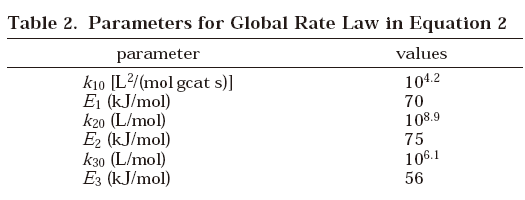
\includegraphics[width=0.8\textwidth]{Q2_ref.png}
    \caption{Parameter Values Reported in Reference for Problem 2[2]}
\end{figure}

By observing figure 5 and 6, one could conclude that GNM and NMA are not predicting the parameters reasonably. Even though for some cases, the estimated X values agree with the experiment data, large error remains in other cases.
The reason could be the complexity of the model and the inability of the code to solve numerically when applying those optimization methods.
\begin{figure}[ht]
    \centering
    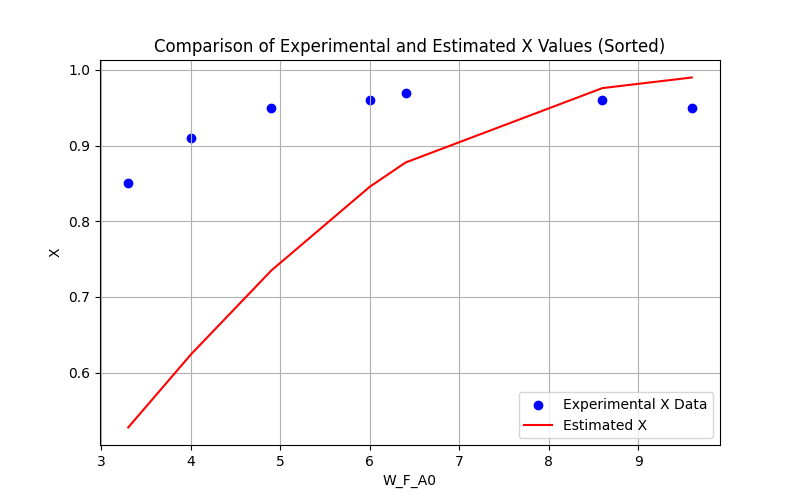
\includegraphics[width=0.8\textwidth]{Q2_GMN_comp.png}
    \caption{Experiment Data vs. Estimated Data of q for Problem 2 by GNM}
\end{figure}
\begin{figure}[ht]
    \centering
    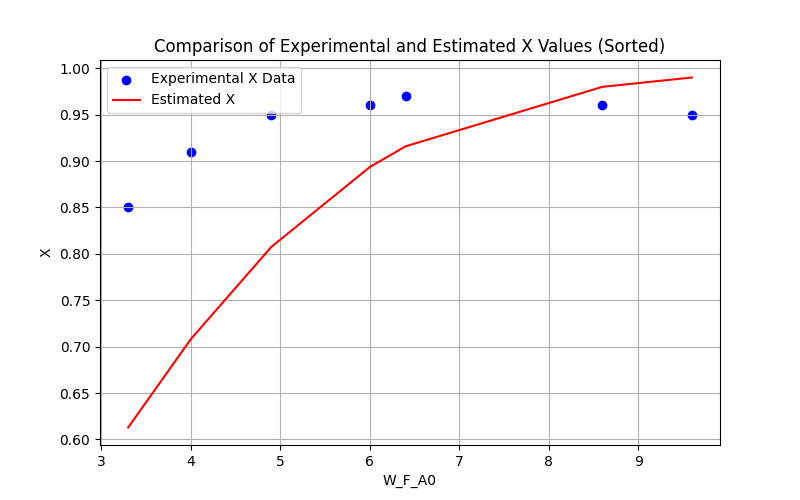
\includegraphics[width=0.8\textwidth]{Q2_NMA_comp.png}
    \caption{Experiment Data vs. Estimated Data of q for Problem 1 by NMA}
\end{figure}

\clearpage
\section{Conclusion}
The investigation into the Gauss-Newton method with Marquardt modification and the Nelder-Mead algorithm revealed distinct differences in their applicability and performance in the context of parameter estimation for complex chemical engineering processes. The Gauss-Newton method, enhanced by Marquardt’s modification, demonstrated high accuracy in parameter estimation for simpler model scenarios but was less effective in handling more complex models with higher parameter uncertainty. On the other hand, the Nelder-Mead algorithm, while generally more robust in dealing with non-linear problems without derivative information, showed limitations in precision and confidence interval estimation, which was mitigated by employing the bootstrap method. Both methods showcased their respective strengths and weaknesses, indicating the necessity for careful selection of optimization techniques based on the model characteristics and data quality. Future work should focus on enhancing these methods for higher complexity models and integrating more advanced statistical tools to improve the reliability and accuracy of parameter estimations in scientific research and industrial applications.
\section{Reference}
\begin{enumerate}
    \item Zhang et al., "Adsorption of 1,2-Dichloropropane on Activated Carbon", J Chem Eng Data, 2001, 46, 662-664.
    \item Yu and Savage, "Kinetics of MnO2-catalysed acetic acid oxidation in supercritical water", Ind. Eng. Chem. Res. 2000, 39, 4014-4019.
\end{enumerate}
\section{Appendix}
\begin{figure}[ht]
    \centering
    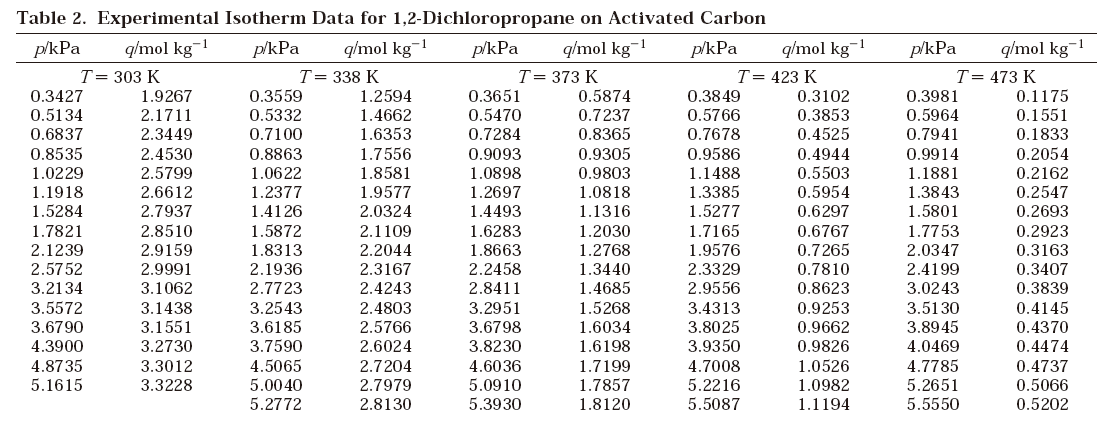
\includegraphics[width=1\textwidth]{Q1_data.png}
    \caption{Experiment Data for Problem 1[1]}
\end{figure}

\begin{figure}[ht]
    \centering
    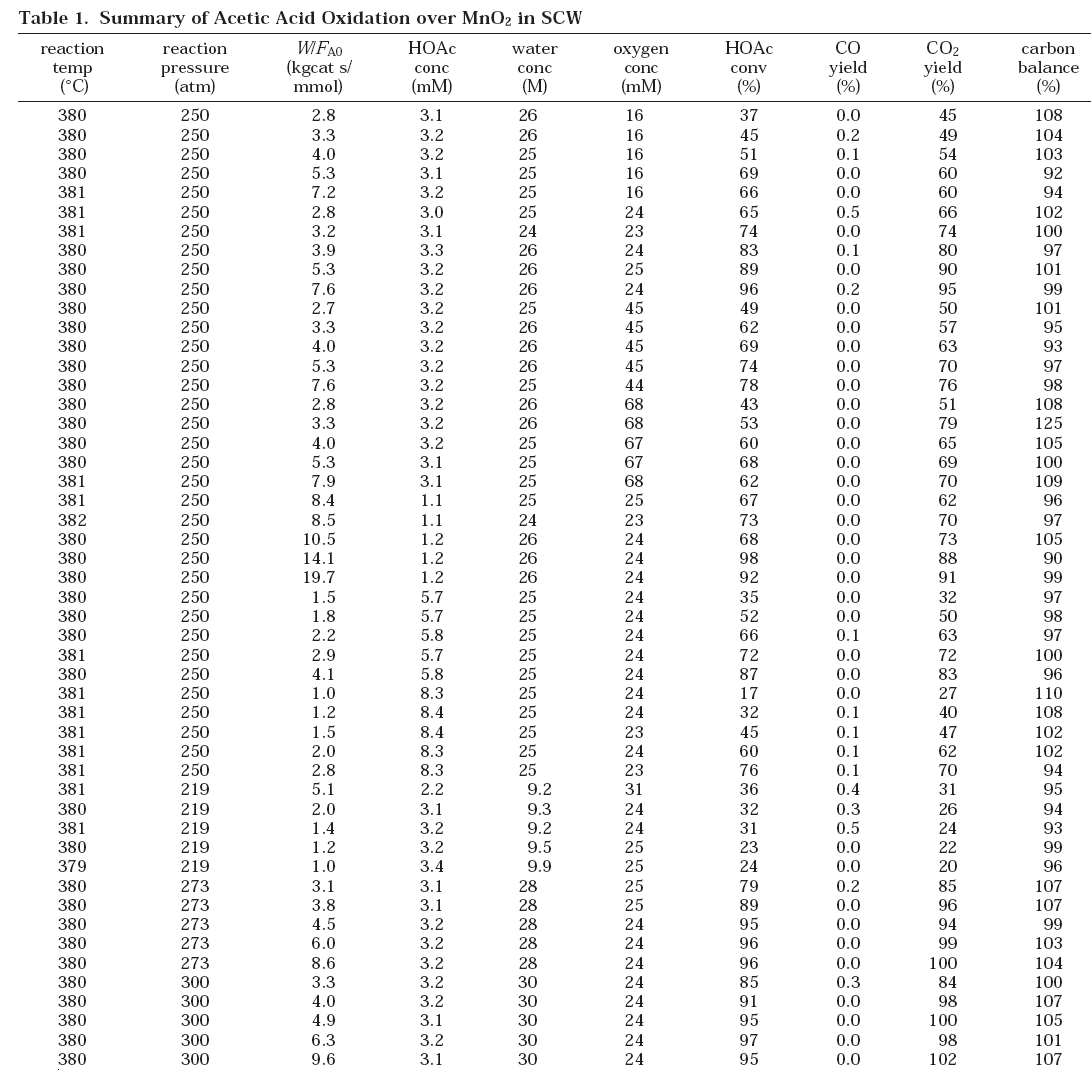
\includegraphics[width=1\textwidth]{Q2_data.png}
    \caption{Experiment Data for Problem 2[2]}
\end{figure}
\end{document}